\documentclass[tikz]{standalone}
\usetikzlibrary{ext.misc}
\begin{document}
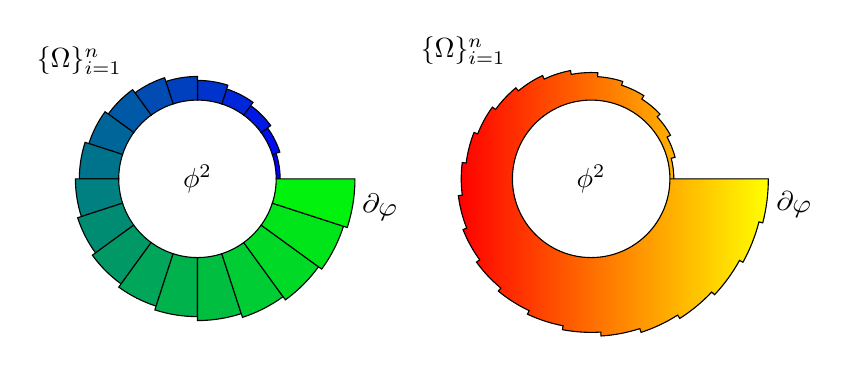
\begin{tikzpicture}[
  declare function={bigR(\n)=smallR+.05*\n;},
  declare constant={smallR=1; segments=20;},
  full arc=segments]
\foreach \iN[evaluate={\endRadius=bigR(\iN+1);}, use int=0 to segments-1]
  \filldraw[fill/.pgfmath wrap={green!##1!blue}{100*\iN/segments}] (\iN R:\endRadius)
    arc [radius=\endRadius, start angle=\iN R, delta angle=+1R] -- (\iN R+1R:smallR)
    arc [radius=smallR,       end angle=\iN R, delta angle=-1R] -- cycle;
\node                                              {$\phi^2$};
\node at (north west:{sqrt 2 * bigR(segments/2)})  {$\{\Omega\}_{i=1}^n$};
\node[rotate=-.5R, right] at (-.5R: bigR segments) {$\partial \varphi$};

\tikzset{xshift=5cm, declare constant={segments=25;}, full arc=segments}
\filldraw[left color=red, right color=yellow] (right:smallR)
  foreach \iN[evaluate={\endRadius=bigR(\iN+1);}, use int=0 to segments-1] {
    -- (\iN R:\endRadius) arc[radius=\endRadius, start angle=\iN R, delta angle=1R]}
    -- (right:smallR)
    arc[radius=smallR, start angle=0, delta angle=-360];
\node                                              {$\phi^2$};
\node at (north west:{sqrt 2 * bigR(segments/2)})  {$\{\Omega\}_{i=1}^n$};
\node[rotate=-.5R, right] at (-.5R: bigR segments) {$\partial \varphi$};
\end{tikzpicture}
\end{document}